\documentclass{article}\usepackage[]{graphicx}\usepackage[]{color}
%% maxwidth is the original width if it is less than linewidth
%% otherwise use linewidth (to make sure the graphics do not exceed the margin)
\makeatletter
\def\maxwidth{ %
  \ifdim\Gin@nat@width>\linewidth
    \linewidth
  \else
    \Gin@nat@width
  \fi
}
\makeatother

\definecolor{fgcolor}{rgb}{0.345, 0.345, 0.345}
\newcommand{\hlnum}[1]{\textcolor[rgb]{0.686,0.059,0.569}{#1}}%
\newcommand{\hlstr}[1]{\textcolor[rgb]{0.192,0.494,0.8}{#1}}%
\newcommand{\hlcom}[1]{\textcolor[rgb]{0.678,0.584,0.686}{\textit{#1}}}%
\newcommand{\hlopt}[1]{\textcolor[rgb]{0,0,0}{#1}}%
\newcommand{\hlstd}[1]{\textcolor[rgb]{0.345,0.345,0.345}{#1}}%
\newcommand{\hlkwa}[1]{\textcolor[rgb]{0.161,0.373,0.58}{\textbf{#1}}}%
\newcommand{\hlkwb}[1]{\textcolor[rgb]{0.69,0.353,0.396}{#1}}%
\newcommand{\hlkwc}[1]{\textcolor[rgb]{0.333,0.667,0.333}{#1}}%
\newcommand{\hlkwd}[1]{\textcolor[rgb]{0.737,0.353,0.396}{\textbf{#1}}}%
\let\hlipl\hlkwb

\usepackage{framed}
\makeatletter
\newenvironment{kframe}{%
 \def\at@end@of@kframe{}%
 \ifinner\ifhmode%
  \def\at@end@of@kframe{\end{minipage}}%
  \begin{minipage}{\columnwidth}%
 \fi\fi%
 \def\FrameCommand##1{\hskip\@totalleftmargin \hskip-\fboxsep
 \colorbox{shadecolor}{##1}\hskip-\fboxsep
     % There is no \\@totalrightmargin, so:
     \hskip-\linewidth \hskip-\@totalleftmargin \hskip\columnwidth}%
 \MakeFramed {\advance\hsize-\width
   \@totalleftmargin\z@ \linewidth\hsize
   \@setminipage}}%
 {\par\unskip\endMakeFramed%
 \at@end@of@kframe}
\makeatother

\definecolor{shadecolor}{rgb}{.97, .97, .97}
\definecolor{messagecolor}{rgb}{0, 0, 0}
\definecolor{warningcolor}{rgb}{1, 0, 1}
\definecolor{errorcolor}{rgb}{1, 0, 0}
\newenvironment{knitrout}{}{} % an empty environment to be redefined in TeX

\usepackage{alltt}
\usepackage{amsmath, amssymb}
\IfFileExists{upquote.sty}{\usepackage{upquote}}{}
\begin{document}
%\SweaveOpts{concordance=TRUE}

\begin{knitrout}
\definecolor{shadecolor}{rgb}{0.969, 0.969, 0.969}\color{fgcolor}\begin{kframe}


{\ttfamily\noindent\itshape\color{messagecolor}{\#\# Registering fonts with R}}

{\ttfamily\noindent\itshape\color{messagecolor}{\#\# Package "{}fontcm"{} already installed.}}

{\ttfamily\noindent\itshape\color{messagecolor}{\#\# Registering font package "{}fontcm"{} with fonts.}}

{\ttfamily\noindent\itshape\color{messagecolor}{\#\# Font package "{}fontcm"{} already registered in fonts database.}}

{\ttfamily\noindent\itshape\color{messagecolor}{\#\# \\\#\# Attaching package: 'dplyr'}}

{\ttfamily\noindent\itshape\color{messagecolor}{\#\# The following objects are masked from 'package:plyr':\\\#\# \\\#\#\ \ \ \  arrange, count, desc, failwith, id, mutate, rename, summarise,\\\#\#\ \ \ \  summarize}}

{\ttfamily\noindent\itshape\color{messagecolor}{\#\# The following objects are masked from 'package:stats':\\\#\# \\\#\#\ \ \ \  filter, lag}}

{\ttfamily\noindent\itshape\color{messagecolor}{\#\# The following objects are masked from 'package:base':\\\#\# \\\#\#\ \ \ \  intersect, setdiff, setequal, union}}\end{kframe}
\end{knitrout}


\section{Description}
The symetric random walk will be described in this document (Mt). it covers the theory of "Stochastic Calculus for finance" Tome 2 chapter 3 section 1.

The construction of the random walk depend on the evolution of a random variable $X_i$. The previous RV can take two value at each time, like tossing a coin. $X_i$ can take the value 1 or -1.

\begin{equation}
 \label{eq:Xi}
X_i = 
\left \{{
  \begin{array}{c} 1 \\ -1 \end{array}
  }\right .
\end{equation}
 
The Symetric Random Walk is constructed by summing up the different outcome of the random variable $X_i$ from $k$ experiments:

\begin{equation}
\label{eq:SRW}
M_k = 
\sum_{j=1}^k X_j
\end{equation}

In the following lines of code, $X_i$ is randomly difined. The variable $k$ ensure to have a sufficent number of periods to further generate the scaled random walk.
It refers to the $k$ of equation~\ref{eq:SRW}.
$p$ and $q$ are the probability measure, respectively $p$ chance to get value 1 and $q$ chance to get -1 from random variable $X_i$.

 


After creating the random variable $X_i$ it suffices to add up all the differente output we get from time 1 up to $k$ to get a specific Symetric Random Walk.

The following outcome present a randomly generated 300 steps symmetric random walk.

\begin{table}[h]

\caption{300 steps Symmetric Random Walk}
\end{table}


\begin{figure}[!h]
\begin{center}

\begin{knitrout}
\definecolor{shadecolor}{rgb}{0.969, 0.969, 0.969}\color{fgcolor}
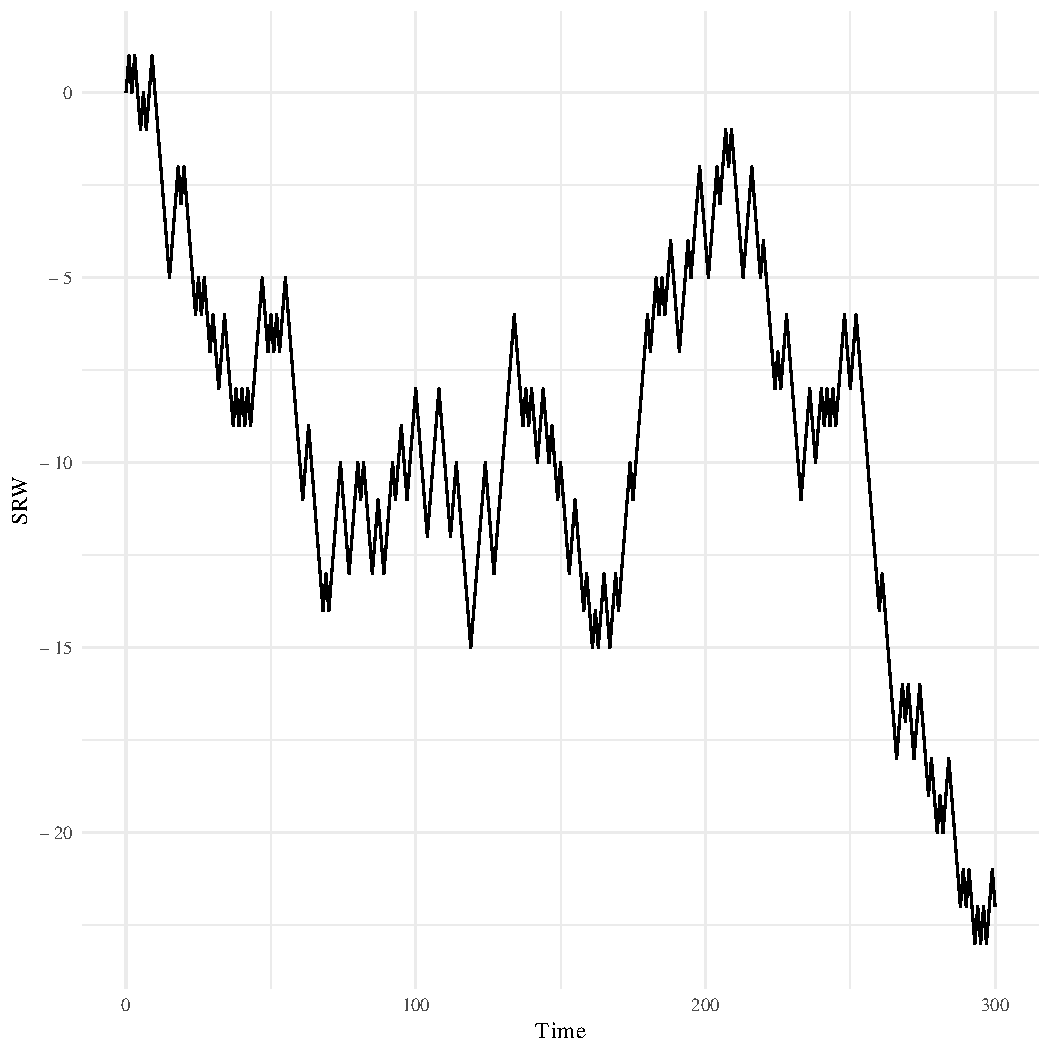
\includegraphics[width=1\linewidth]{figure/unnamed-chunk-4-1} 

\end{knitrout}


\end{center}
\caption{Symmetric Random Walk}
\end{figure}

\begin{kframe}
\begin{alltt}
\hlcom{# Because squared matrix dim(y) = dim(x):}
\hlstd{dim_x} \hlkwb{<-} \hlstd{dim_y} \hlkwb{<-} \hlnum{1}\hlopt{:}\hlstd{(k} \hlopt{+} \hlnum{1}\hlstd{)} \hlcom{# from 1 to k+1 because we start to time zero nonrandom which equal to zero}
\hlstd{o} \hlkwb{<-} \hlkwd{outer}\hlstd{(dim_x, dim_y,} \hlkwc{FUN}\hlstd{=}\hlkwa{function}\hlstd{(}\hlkwc{r}\hlstd{,}\hlkwc{c}\hlstd{)\{(r}\hlopt{-}\hlstd{c)} \hlopt{+} \hlstd{(}\hlnum{1}\hlopt{-}\hlstd{c)\} )}
\hlstd{to} \hlkwb{<-} \hlkwd{t}\hlstd{(o)}
\hlstd{subset} \hlkwb{<-} \hlkwd{upper.tri}\hlstd{(to,} \hlkwc{diag} \hlstd{= T)}
\hlstd{Mk} \hlkwb{<-} \hlstd{to} \hlopt{*} \hlstd{subset}
\hlkwd{colnames}\hlstd{(Mk)} \hlkwb{<-} \hlkwd{paste0}\hlstd{(}\hlstr{"F("}\hlstd{,} \hlnum{1}\hlopt{:}\hlkwd{ncol}\hlstd{(Mk)} \hlopt{-} \hlnum{1}\hlstd{,} \hlstr{")"}\hlstd{)}
\hlcom{# Transform Mk to better suit the table:}
\hlstd{Mk_print} \hlkwb{<-} \hlkwd{apply}\hlstd{(Mk,} \hlnum{2}\hlstd{, as.character)}
\hlcom{# Create the Tex Table > tabular}
\hlstd{Mk.tab} \hlkwb{<-} \hlkwd{xtable}\hlstd{(Mk_print[}\hlnum{1}\hlopt{:}\hlnum{10}\hlstd{,} \hlnum{1}\hlopt{:}\hlnum{10}\hlstd{],} \hlkwc{digits} \hlstd{=} \hlnum{0}\hlstd{,} \hlkwc{format} \hlstd{=} \hlstr{"latex"}\hlstd{)}
\hlkwd{align}\hlstd{(Mk.tab)} \hlkwb{<-} \hlkwd{rep}\hlstd{(}\hlstr{"r"}\hlstd{,} \hlnum{11}\hlstd{)}
\hlstd{Mk.tab}
\end{alltt}
\end{kframe}% latex table generated in R 3.4.0 by xtable 1.8-2 package
% Wed May 17 11:00:34 2017
\begin{table}[ht]
\centering
\begin{tabular}{rrrrrrrrrrr}
  \hline
 & F(0) & F(1) & F(2) & F(3) & F(4) & F(5) & F(6) & F(7) & F(8) & F(9) \\ 
  \hline
1 & 0 & 1 & 2 & 3 & 4 & 5 & 6 & 7 & 8 & 9 \\ 
  2 & 0 & -1 & 0 & 1 & 2 & 3 & 4 & 5 & 6 & 7 \\ 
  3 & 0 & 0 & -2 & -1 & 0 & 1 & 2 & 3 & 4 & 5 \\ 
  4 & 0 & 0 & 0 & -3 & -2 & -1 & 0 & 1 & 2 & 3 \\ 
  5 & 0 & 0 & 0 & 0 & -4 & -3 & -2 & -1 & 0 & 1 \\ 
  6 & 0 & 0 & 0 & 0 & 0 & -5 & -4 & -3 & -2 & -1 \\ 
  7 & 0 & 0 & 0 & 0 & 0 & 0 & -6 & -5 & -4 & -3 \\ 
  8 & 0 & 0 & 0 & 0 & 0 & 0 & 0 & -7 & -6 & -5 \\ 
  9 & 0 & 0 & 0 & 0 & 0 & 0 & 0 & 0 & -8 & -7 \\ 
  10 & 0 & 0 & 0 & 0 & 0 & 0 & 0 & 0 & 0 & -9 \\ 
   \hline
\end{tabular}
\end{table}


\begin{knitrout}
\definecolor{shadecolor}{rgb}{0.969, 0.969, 0.969}\color{fgcolor}\begin{kframe}
\begin{alltt}
\hlcom{# compute the probability measure to apply on the Random Variable Mk}
\hlstd{fi} \hlkwb{<-} \hlkwd{outer}\hlstd{(dim_x,}
            \hlstd{dim_y,}
            \hlkwc{FUN} \hlstd{=} \hlkwa{function}\hlstd{(}\hlkwc{i}\hlstd{,} \hlkwc{j}\hlstd{)\{}\hlkwd{choose}\hlstd{((j}\hlopt{-}\hlnum{1}\hlstd{), (j}\hlopt{-}\hlstd{i))} \hlopt{*} \hlstd{p}\hlopt{^}\hlstd{(j}\hlopt{-}\hlnum{1}\hlstd{)\})}
\end{alltt}
\end{kframe}
\end{knitrout}

\begin{knitrout}
\definecolor{shadecolor}{rgb}{0.969, 0.969, 0.969}\color{fgcolor}\begin{kframe}
\begin{alltt}
 \hlstd{range} \hlkwb{<-} \hlnum{1}\hlopt{:}\hlkwd{ncol}\hlstd{(Mk)}
\hlstd{lastToss} \hlkwb{<-} \hlkwd{ncol}\hlstd{(Mk)}
 \hlcom{# Using ggplot}
\hlcom{# data.frame which map distribution and random variable:}
\hlstd{distributionSymRanWal} \hlkwb{<-} \hlkwd{data.frame}\hlstd{(}
  \hlkwc{Value} \hlstd{= Mk[range, lastToss],}
  \hlkwc{Frequency} \hlstd{= fi[range, lastToss]}
\hlstd{)}

\hlcom{# For the sake of visibility the limit of X axis has been set to [-100, 100]}
\hlkwd{ggplot}\hlstd{(}\hlkwc{data} \hlstd{= distributionSymRanWal,} \hlkwd{aes}\hlstd{(Value, Frequency))} \hlopt{+}
  \hlkwd{geom_line}\hlstd{()} \hlopt{+}
  \hlkwd{scale_x_continuous}\hlstd{(}\hlkwc{limits} \hlstd{=} \hlkwd{c}\hlstd{(}\hlopt{-}\hlnum{100}\hlstd{,} \hlnum{100}\hlstd{))} \hlopt{+}
   \hlkwd{theme_minimal}\hlstd{()} \hlopt{+}
  \hlkwd{theme}\hlstd{(}\hlkwc{text} \hlstd{=} \hlkwd{element_text}\hlstd{(}\hlkwc{family}\hlstd{=}\hlstr{"CM Roman"}\hlstd{),}
        \hlkwc{axis.title} \hlstd{=} \hlkwd{element_text}\hlstd{(}\hlkwc{face} \hlstd{=} \hlstr{"plain"}\hlstd{))}
\end{alltt}


{\ttfamily\noindent\color{warningcolor}{\#\# Warning: Removed 200 rows containing missing values (geom\_path).}}\end{kframe}
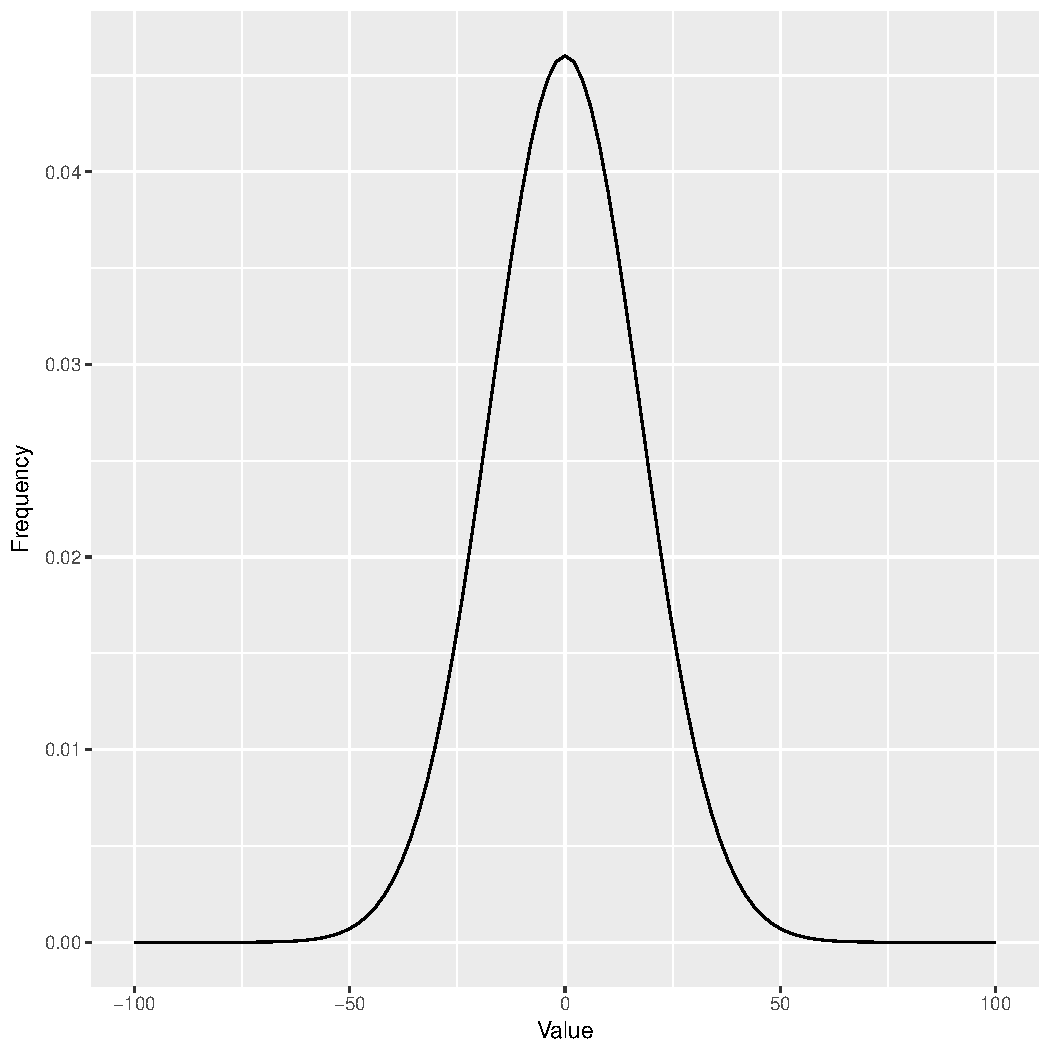
\includegraphics[width=\maxwidth]{figure/unnamed-chunk-7-1} 

\end{knitrout}


\section{Martingale property}

\begin{equation}
\mathop{\mathbb{E}}[X] = \sum_{i=1}^N p_i \times x_i
\end{equation}

To show the martingale property we have to show that the expectation of the symmetric random walk $\mathop{\mathbb{E}}[X|F(0)] = M_0 = 0$

\begin{knitrout}
\definecolor{shadecolor}{rgb}{0.969, 0.969, 0.969}\color{fgcolor}\begin{kframe}
\begin{alltt}
 \hlstd{EM200} \hlkwb{=} \hlkwd{sum}\hlstd{(Mk[}\hlnum{1}\hlopt{:}\hlnum{200}\hlstd{,} \hlnum{200}\hlstd{]} \hlopt{*} \hlstd{fi[}\hlnum{1}\hlopt{:}\hlnum{200}\hlstd{,} \hlnum{200}\hlstd{])} \hlcom{# equal zero.}
\end{alltt}
\end{kframe}
\end{knitrout}




 
           
\end{document}
